%%%%%%%%%%%%%%%%%%%%%%%%%%%%%%%%%%%%%%%%%
% Arsclassica Article
% LaTeX Template
% Version 1.1 (10/6/14)
%
% This template has been downloaded from:
% http://www.LaTeXTemplates.com
%
% Original author:
% Lorenzo Pantieri (http://www.lorenzopantieri.net) with extensive modifications by:
% Vel (vel@latextemplates.com)
%
% License:
% CC BY-NC-SA 3.0 (http://creativecommons.org/licenses/by-nc-sa/3.0/)
%
%%%%%%%%%%%%%%%%%%%%%%%%%%%%%%%%%%%%%%%%%

%----------------------------------------------------------------------------------------
%	PACKAGES AND OTHER DOCUMENT CONFIGURATIONS
%----------------------------------------------------------------------------------------

\documentclass[
10pt, % Main document font size
letterpaper, % Paper type, use 'letterpaper' for US Letter paper
oneside, % One page layout (no page indentation)
%twoside, % Two page layout (page indentation for binding and different headers)
headinclude,footinclude, % Extra spacing for the header and footer
english
]{article}

%%%%%%%%%%%%%%%%%%%%%%%%%%%%%%%%%%%%%%%%%
% Arsclassica Article
% Structure Specification File
%
% This file has been downloaded from:
% http://www.LaTeXTemplates.com
%
% Original author:
% Lorenzo Pantieri (http://www.lorenzopantieri.net) with extensive modifications by:
% Vel (vel@latextemplates.com)
%
% License:
% CC BY-NC-SA 3.0 (http://creativecommons.org/licenses/by-nc-sa/3.0/)
%
%%%%%%%%%%%%%%%%%%%%%%%%%%%%%%%%%%%%%%%%%

%----------------------------------------------------------------------------------------
%	REQUIRED PACKAGES
%----------------------------------------------------------------------------------------

\usepackage[
nochapters, % Turn off chapters since this is an article        
beramono, % Use the Bera Mono font for monospaced text (\texttt)
eulermath,% Use the Euler font for mathematics
pdfspacing, % Makes use of pdftex’ letter spacing capabilities via the microtype package
dottedtoc % Dotted lines leading to the page numbers in the table of contents
]{classicthesis} % The layout is based on the Classic Thesis style

\usepackage{arsclassica} % Modifies the Classic Thesis package

\usepackage[T1]{fontenc} % Use 8-bit encoding that has 256 glyphs

\usepackage[utf8]{inputenc} % Required for including letters with accents

\usepackage{graphicx} % Required for including images
\graphicspath{{Figures/}} % Set the default folder for images

\usepackage{enumitem} % Required for manipulating the whitespace between and within lists

\usepackage{lipsum} % Used for inserting dummy 'Lorem ipsum' text into the template

\usepackage{subfig} % Required for creating figures with multiple parts (subfigures)

\usepackage{amsmath,amssymb,amsthm} % For including math equations, theorems, symbols, etc

\usepackage{varioref} % More descriptive referencing

%----------------------------------------------------------------------------------------
%	THEOREM STYLES
%---------------------------------------------------------------------------------------

\theoremstyle{definition} % Define theorem styles here based on the definition style (used for definitions and examples)
\newtheorem{definition}{Definition}

\theoremstyle{plain} % Define theorem styles here based on the plain style (used for theorems, lemmas, propositions)
\newtheorem{theorem}{Theorem}

\theoremstyle{remark} % Define theorem styles here based on the remark style (used for remarks and notes)

%----------------------------------------------------------------------------------------
%	HYPERLINKS
%---------------------------------------------------------------------------------------

\hypersetup{
%draft, % Uncomment to remove all links (useful for printing in black and white)
colorlinks=true, breaklinks=true, bookmarks=true,bookmarksnumbered,
urlcolor=webbrown, linkcolor=RoyalBlue, citecolor=webgreen, % Link colors
pdftitle={}, % PDF title
pdfauthor={\textcopyright}, % PDF Author
pdfsubject={}, % PDF Subject
pdfkeywords={}, % PDF Keywords
pdfcreator={pdfLaTeX}, % PDF Creator
pdfproducer={LaTeX with hyperref and ClassicThesis} % PDF producer
} % Include the structure.tex file which specified the document structure and layout
\usepackage[letterpaper]{geometry}
\geometry{verbose,tmargin=1in,bmargin=1.3in,lmargin=1.5in,rmargin=1.5in}

\hyphenation{Fortran hy-phen-ation} % Specify custom hyphenation points in words with dashes where you would like hyphenation to occur, or alternatively, don't put any dashes in a word to stop hyphenation altogether

%----------------------------------------------------------------------------------------
%	TITLE AND AUTHOR(S)
%----------------------------------------------------------------------------------------

\title{\normalfont\spacedallcaps{CIS 559 Project 2:\break Parallel Football}} % The article title

\author{\spacedlowsmallcaps{Ian Sibner, Michael Molisani, and Laura Kingsley}} % The article author(s) - author affiliations need to be specified in the AUTHOR AFFILIATIONS block

\date{20 October 2015} % An optional date to appear under the author(s)

%----------------------------------------------------------------------------------------
\setlength\parindent{0pt}
\setlength{\parskip}{1em}

\usepackage[section]{placeins}

\begin{document}

%----------------------------------------------------------------------------------------
%	HEADERS
%----------------------------------------------------------------------------------------

\renewcommand{\sectionmark}[1]{\markright{\spacedlowsmallcaps{#1}}} % The header for all pages (oneside) or for even pages (twoside)
%\renewcommand{\subsectionmark}[1]{\markright{\thesubsection~#1}} % Uncomment when using the twoside option - this modifies the header on odd pages
\lehead{\mbox{\llap{\small\thepage\kern1em\color{halfgray} \vline}\color{halfgray}\hspace{0.5em}\rightmark\hfil}} % The header style

\pagestyle{scrheadings} % Enable the headers specified in this block

%----------------------------------------------------------------------------------------
%	TABLE OF CONTENTS & LISTS OF FIGURES AND TABLES
%----------------------------------------------------------------------------------------

\maketitle % Print the title/author/date block

\setcounter{tocdepth}{2} % Set the depth of the table of contents to show sections and subsections only

\tableofcontents % Print the table of contents

\listoffigures % Print the list of figures

% \listoftables % Print the list of tables

%----------------------------------------------------------------------------------------
%	ABSTRACT
%----------------------------------------------------------------------------------------

\section{Introduction} % This section will not appear in the table of contents due to the star (\section*)

The Organisms game consists of a world (an $m \times n$) grid populated by one or more organisms. Each organism has a \textit{brain} (its controlling program) and an \textit{energy level}. An organism expends energy each turn - 1 unit to stay in the same place, and some variable amount of energy $v$ to move to one of its four unoccupied neighbor squares (up, right, down, and left). Moving off the board is allowed; the world wraps around and the organism simply appears on the opposite side. An organism gains energy by eating food, which has some probability of spontaneously appearing on an empty cell. Multiple units of food can occupy a given cell, up to some threshold, and each turn a unit of food in a cell which is not occupied by an organism has a chance of doubling (so a cell with three units of food may have anywhere from 3 to 6 units the next turn depending on randomness). An organism can also \textit{reproduce} onto an adjacent empty square at the cost of $v$ energy. Each unit will have half of the organism's remaining energy after paying the reproduction cost.

The parameters of the simulation are listed below:

\begin{tabular}{|c|c|}
\hline
\textbf{Parameter} & \textbf{Meaning}\\ \hline
$m$ & Horizontal board size (X-direction) \\ \hline
$n$ & Vertical board size (Y-direction) \\ \hline
$p$ & Chance of food spontaneously appearing in an unoccupied space \\ \hline
$q$ & Chance that a given unit of food in an unoccupied space will double \\ \hline
$v$ & Energy consumed by moving or reproducing \\ \hline
$u$ & Energy gained by an organism for consumption of one unit of food \\ \hline
$M$ & Maximum energy level for an organism \\ \hline
$K$ & Maximum number of food units per cell \\ \hline
\end{tabular}

Additionally, an organism has a \textit{state} (an integer between 0 and 255) which it can set each turn it acts. An organism can only ``see'' in four directions (up, right, down, and left). It can sense the amount of food in its current cell, the presence of food in the four neighboring cells (but not the amount), and the presence and state of any organism in the neighboring cells. Organisms are aware of only a limited subset of parameter values ($v$, $u$, $M$, and $K$) but not the others.

Each turn, an organism can change its state, stay put, move, or reproduce. Moves are calculated row-by-row, from top to bottom; this means that an organism at (1,1) will move before an organism at (2,1). If a move is not valid (possibly because another organism moved into a previously unoccupied space before another could act), then it is treated as a stay-put move.

\section{Initial Insights and Observations}

Immediately, our team observed several key features about the game.

\begin{enumerate}
  \item The information available to organisms would be very limited. They can only `see' in four directions, and could only detect food (or lack of food) and other organisms' states. So strategies that required non-local knowledge or multi-organism coordination would be difficult to implement.
  \item Staying put is much cheaper than moving since $v \geq 1$. Also, for the majority of the setups we considered, we had $v \geq 20$. Therefore, an organism should stay put more often than it moves.
  \item For all setups, we had $q \geq p$. This means that food tended to `collect' in certain squares, rather than being widely distributed on empty squares.
  \item A player with fewer individual organisms tends to die out faster, due to the random nature of food spawning. So it pays to try and reproduce.
  \item Reproducing produces two organisms with half the energy of the original, so the more energy an organism has when it reproduces, the more likely both offspring will survive.
\end{enumerate}

These insights guided our strategy throughout and allowed us to focus on the most important aspects of the game.

\section{Strategies and Concepts}

\subsection {XOrganism}

XOrganism was our first attempt, so we tried to create an organism that would survive on its own in a variety of conditions. The goal was to have a good survival rate in ``desert'' conditions, where $p \leq 0.005$. We did this in several ways.

First, we defined the idea of an organism being `sated'. In effect, a sated organism is close enough to its maximum energy that it is not in immediate need of food. There are many possible definitions for satiety; we initially defined an organism as sated if $Energy_{organism} \geq M - u$. This was a fairly intuitive definition: an organism is sated if eating one more unit of food would fill it up completely.

For movement, we tried to stay put very often because it only cost 1 unit of energy. We only moved under a few conditions:
\begin{enumerate}
  \item An adjacent square has food, and the organism is not `sated'. The rationale behind this movement pattern is fairly obvious - organisms tend to survive longer if they seek out food.
  \item The organism is `sated', but its square still has food. The idea here was to be \textit{courteous}, and allow other organisms who might need that food to jump on it.
  \item The organism has not found food in 20 turns. In this case, it moves in a random direction to try to look for food it might have missed.
\end{enumerate}
For reproduction, our organism was similarly simple. If the player is sated, then there is a 70\% chance of reproducing in a random direction. This ensures that when an organism does reproduce, both offspring have about half of their maximum energy, giving them a better chance of survival.

This organism tended to do pretty well on its own, surviving in about 30\% of our test runs with $p=0.005$. However, it performed significantly worse than other players in configurations where food was readily available. Worse, it tended to get ``choked out'' by more aggressive players, who would often take advantage of its courteous moves to take the food for themselves and reproduce. So, while it was a fairly good start, we needed to make some changes before XOrganism could be competitive.

\subsection{Protective Farmer}
The benefit function was inspired by what we thought a human player would consider while deciding where best to move. We realized that given a point on the board, factors considered while deciding whether or not to move towards that point included not only the Euclidean distance to that point, but also the number of opponents, concentration of balls in the general vicinity of that point, and distance of that point from our home goal. Accounting for the proximity of opponents was particularly important becuase it gave us a measure of how susceptible to change the benefit of a particular cell was: the nearer the opponents, and the higher the number of opponents, the more likely it was for balls in the cell in question to be kicked out. This allowed us to take into consideration not just how the board was laid out now, but also gave us a proxy for how each cell might change in the near future.

The following is the benefit function for each cell that was calculated from the perspective of each player on the board so as to allow for the player to move to the cell that offered him the greatest benefit:
$$B_{i, j} = G_{i, j} - D_{i,j} $$

where $G_{i, j}$ is the gain offered by that cell and its neighboring $4 \times 4$ cluster of cells to the player and $D_{i, j}$ is the distance penalty for that cell given the position of the player and the cell. $$G_{i, j} = \sum_{a : |a - i| \leq 2}\ \ \sum_{b : |b - j| \leq 2} \alpha \times numBalls(cell_{i, j}) - \beta \times numOpponents(cell_{i,j}) $$ and $$D_{i, j} = \gamma \times cellDistanceFromPlayer(cell_{i,j}) + \delta \times numKicksFromCellToOurHomeGoal(cell_{i, j})$$ where $\alpha = 1.2$, $\beta = 0.4$, $\gamma = 1$ and $\delta = 5$ are weights. These weights were assigned based on the optimal values we found through emperical observations of our performance against other teams over a range of weights.

\subsection{SimplePlayer}
On the second iteration of our benefit function, we accounted for ball and opponent clustering by keeping track of the number of balls and opponents surrounding a particular cell. This allowed our players to seek out areas of high benefit, rather than single cells.

After initial trials with a large radius, we settled on a radius of 4. We observed that larger radii caused the players to move back and forth somewhat inefficiently, and hypothesize that these larger zones changed too quickly for players to capitalize on them.

\section{Implementation}

\subsection{XOrganism}

The implementation of XOrganism was fairly straightforward, as it only considered its current energy level and known parameter values. The only bit of state that was carried over (in addition to game state, such as current energy level) was the number of turns it had been alive (which was used in order to move every 20th turn to seek out more food). We first defined an \texttt{isSated} function (which just determined whether $Energy_{organism} \geq M - u$). Then, every turn, we did the following:

\begin{enumerate}
  \item If the organism was sated, we would reproduce with a probability of 70\%.
  \item If the organism did not reproduce, but still had food on its square and was sated, then it would move into an empty adjacent square - a courteous move designed to help other XOrganisms who might need food.
  \item If there was no food in its square, and the organism was not sated, then it would attempt to move into an adjacent square with food. Usually, if there was no food available, the organism would stay put. But every 20th turn (determined by the age counter), it would make a random move in order to seek out pockets of food that might be just beyond its field of vision.
\end{enumerate}

This implementation was very simple - only 100 lines of Java code. This is notable because this organism did tend to survive on its own, showing that even very simple heuristics can lead to acceptable results.

\subsection{Protective Farmer}
In the early phases, we enumerated the different placement strategies and switched according to values of P and K. Our final implementation was fairly simple, and consisted of a random placement of players near the homegoal, with a bounded parameter on $k$ determining their range.

By starting in a tight cluster bounded by the square from our goal out $MIN(K,10)$ spaces, our players would fan out across the board, while the kicking algorithm led to a trail of $k$-spaced players who formed a bucket brigade. The relatively small square space for player placement was chosen as it balanced the advantages of fanning outward from the goal with scoring an initial $k$-distanced ball for each player.

\subsection{SimplePlayer}
As we found through our trials, using a benefit function to determine where a player should go runs into problems when players want to go to the same cell. The players will eventually converge and go to the same cells the rest of the game. To prevent this major inefficency, we implemented a locking mechanism where only one player can go after a single cell at a time. However, we found that although this works great through most of the game, when the number of balls is very small, it becomes better for multiple players to go after the same ball to have a higher likelyhood of kicking the ball to the goal. As such, when the number of balls reaches the number of players on the field, we turn off the locking mechanism.

After only locking the cell that the player is going towards, we also lock a radius around that cell. This allows us to create zones such that only one player clearing a zone.Through experimentation, we found that choosing a radius of max(0,3-P/10) works well. With higher number of players, the smaller the zones should become because there is not enough space to create so many zones. Addditionally, it is more likely that opponents will steal balls from a particular zone before a single player can clear that zone out.

\section{Results}
Generally speaking, we had mixed results. Our rank ranged from $1^{st}$ to $7^{th}$ place. Our most common standing was $3^{rd}$ place. We observed that scores followed relative rank, so we chose rank as the proxy for overall performance in the tournaments.

The overall trend in our performance was that we did better than average given low-to-moderate $k$-values (less than 15), and any $p$-values. This makes sense in terms of our initial placement strategy. With very high values of $k$ (at least 30), our players simply started too close to our goal, and did not take advantage of the potential for long-range kicking. Teams starting in the middle were able to clear balls in a single kick, so that even when our players reached the middle sections quickly, there were few balls left. Contrarily, our players remained competitive with smaller $k$. We think that starting players near the goal led to more effective bucket brigading as described in the initial placement section above. Larger values of $p$ did not have a major impact on performance because more players allowed for a more effective covering of the map while maintaining a bucket brigade path back to the goal. It is possible that parameterizing our intitial placement by $p$ as well as $k$ could have improved our scores, but it may have negatively impacted the bucket brigading, and led to similar results.

Two notable configurations are $P,K=45,1$ and $P,K=30,1$. We placed third and first in these categories, respectively. This was a surprise to us, as we had not optimized for single-player configurations at all. We attribute our success here to the globally-optimal strategy we adopted, so that in slower games with long ranges, our player was able to seek out the most beneficial balls and ball clusters across the entire map. This is in contrast with games with higher $p$, where the board layout changed so rapidly that a global-optimized strategy did not provide much benefit.

Our results are summarized in the following figures.

\begin{figure}[h]
\centering
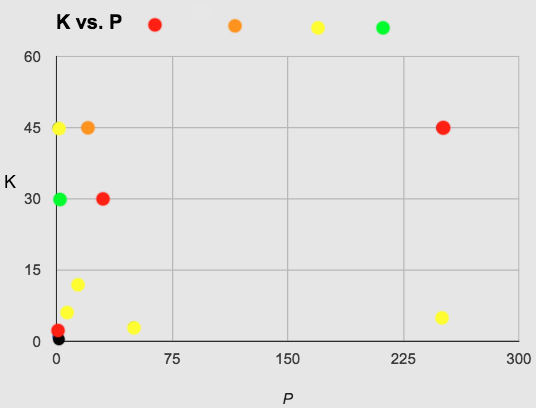
\includegraphics[width=0.8\columnwidth]{results-graph}
\caption[Group 5 tournament results as a function of P and K]{P on the horizontal vs K on the vertical axis. Observe the yellow $3^{rd}$ place band for low $k$}
\label{fig:gallery2}
\end{figure}

\begin{figure}[h]
\centering
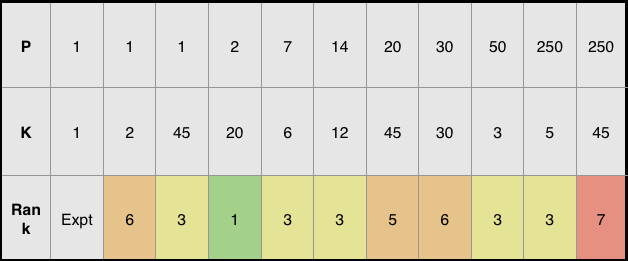
\includegraphics[width=0.8\columnwidth]{results-table}
\caption[Table of rankings per configuration]{Table of rankings per configuration}
\label{fig:gallery2}
\end{figure}

\section{Contributions}

Just as we adopted many good ideas by other teams (see Acknowledgements section), we contributed two major ideas to the group discussion over the course of the project:

\begin{enumerate}
  \item \textbf{Benefit function - } Modelling how a human player would have made his/her movement decision gave us some key insights, especially with the realization that the runtime efficiency of our decision algorithm was not a constraint since this was only a $32 \times 32$ board. We realized that each player on the team could survey the entire board at every time-step and make a player-specific decision of where best to move, taking into account information about ball positions, opponents' positions as well as teammates' current and future positions. In the week after we brought up these insights in class, we saw that many other groups also adopted similar hotspot strategies (i.e. strategies that surveyed the board and picked out the best places to move towards). We were pleased to see that this was an insight that persisted through all further discussions in class and was validated, in different forms, through the strategies of various other teams.
  \item \textbf{Composable Players and Game Phases - } Although we realized early on that the game would likely be characterized by distinct phases in which certain strategies would dominate, it was not until week 2 when other groups really started to pay attention to this idea. This was largely because our performance that week was extremely dominant after we composed \texttt{GridPlayer} in the early game and \texttt{DerickPlayer} for the rest of the round! Other groups began to think about how they could tailor their strategy to perform well in all phases of the game, or at leasthold their own. One group even took this idea to the extreme, creating a \texttt{ReinforcementLearningPlayer} that essentially composed \textit{all} players using a 1NN algorithm!
\end{enumerate}

\section{Future Directions and Limitations}

\subsection{Faster Initial Spread}

Our players tended to do best on larger boards because of its high energy density. It tended not to overextend, unlike some other organisms which would tend to start dying frequently due to very aggressive population growth. But on small maps, this aggressive overextension was actually beneficial to these organisms, because they could ``choke out'' less aggressive competitors and dominate all food resources. Once their opponents went extinct, their organisms would settle into a steady state of lower population and energy compared to their initial population explosion. However, by that time, it was too late for slower-growing competitors like SimplePlayer.

Although an organism might not know the size of the board it starts on, we believe that our SimplePlayer could benefit from employing a more aggressive strategy \textit{only during the first part of the game}. The ideal length of this ``aggressive period'' might vary based on known map conditions, but based on our observations of population explosions in configurations where the total grid size was less than 1000, we believe that around 100 turns of aggressive expansion is usually sufficient to gain dominance over a large portion of the map. Once this period is up, we would switch to our current, more conservative strategy to take advantage of its natural tendency towards higher energy density. This would make our SimplePlayer much harder to choke out at the beginning, but would still allow it to take advantage of its effective conservative strategy after the intial territory grab. Following the initial population explosion, organisms that maintained aggression would tend to move more and use more energy, which would allow our less aggressive organisms to slowly chip away at their territory while maintaining a high average energy level.

\section{Acknowledgments}

The evolution of our players was heavily based on class discussion and iteration of our original ideas based on in-class runs. Group 2 was particularly helpful, due to its ``Rabbits'' strategy (later renamed to ``Harvey''). Their fast expansion - and the way they efficiently choked out our XOrganism and our first draft of SinglePlayer - convinced us of the need to be less cautious about our reproduction chances if we wanted to compete in high-food environments.

\section{Conclusion}

Overall we were happy with the progression of this project, particularly our SimplePlayer's performance on large boards or boards with high movement costs. We ended up with the highest population and overall energy in several of the tournament configurations, showing that good results could be achieved even with comparatively simple heuristics.
\end{document}
